\fontfamily{ptm}\selectfont
\pagenumbering{arabic}
\section*{I. INTRODUCTION}
\addcontentsline{toc}{section}{I.\hspace{0.25in}Introduction}
\begin{flushleft}
	\hspace{0.25in}
	Flowcell sensors have many applications; disease detection, refractive index measurements and measurements of reactivity to name a few. These sensors have been operating on the basis of electromagnetic surface phenomena for decades \cite{homola1999surface}. Most flowcells on the market work by exploiting surface plasma oscillations (SPOs). These oscillations are highly sensitive to changes in the optical properties of the adjacent medium and follow from Maxwell's equations when the dielectric functions of each medium satisfy the relation \cite{JLTROB:1}

	\[
		\frac{\epsilon_{spo}}{\epsilon_{adjacent}} < -1
	\]
	\hspace{0.25in}
	Metals like aluminum, copper, gold, and silver have negative dielectric functions at wavelengths in the red/infrared \cite{JLTROB:1}, so films of these metals are used as to generate SPOs in most flowcell sensors via a process known as Surface Plasmon Resonance (SPR). An SPR system utilizes light-prism coupling to excite the surface electrons on a thin metal film deposited on the hypotenusal face of the prism.
	\begin{figure}[h]
		\begin{center}
			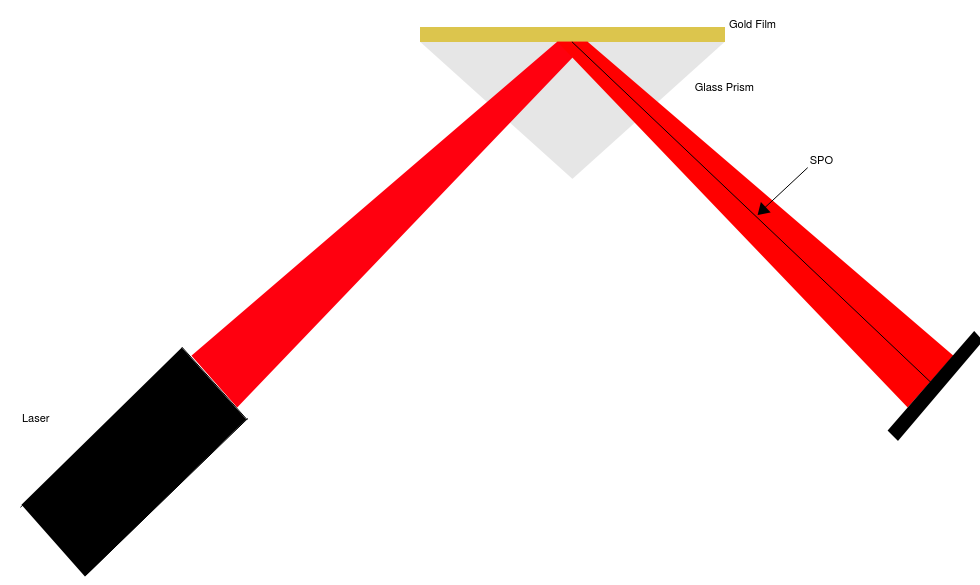
\includegraphics[width=5in]{spr.png}
			\caption{Surface Plasmon Resonance setup}
			\label{fig:SPR}
		\end{center}
	\end{figure}
	A dark band representing the photons absorbed by the surface electrons appears on the reflected beam image as seen in figure \ref{fig:SPR}. There are quite a few drawbacks for using metal films, however. Metals are highly reactive so each time an SPR system is used a new prism must be used. These films also require particular wavelengths of incident light to excite the oscillations. Rather than using metal films, one-dimensional photonic crystals, or multilayers, can be designed to exhibit the phenomenon of surface electromagnetic waves (SEWs) or Bloch surface waves (BSWs), named after the physicist Felix Bloch who was famous for working with periodic systems. These surface waves have the same practical application as SPOs. Multilayers overcome both of the shortcomings of metal films listed here. They can be designed to work for any wavelength and are typically made of nonreactive glass. Modular 3-D printed parts synthesize nicely with the flexible nature of multilayers, resulting in a sensor that is capable of working with many materials. In addition to these benefits, we expect that our 3-D printed and multilayer-based flowcell sensor will be more sensitive and precise with its measurements and be far cheaper to both build and maintain compared to traditional SPR sensors.

	\hspace{0.25in}
	To take measurements with our sensor we look at the reflected image of incident laser light which has been coupled into the prism-multilayer interface to produce a BSW in the terminating layer. Our multilayer is designed to trap incident light in the last layer at a special angle; this results in a dark band in our reflected image. A diagram of the sensor is shown below.

	\begin{figure}[h]
		\begin{center}
			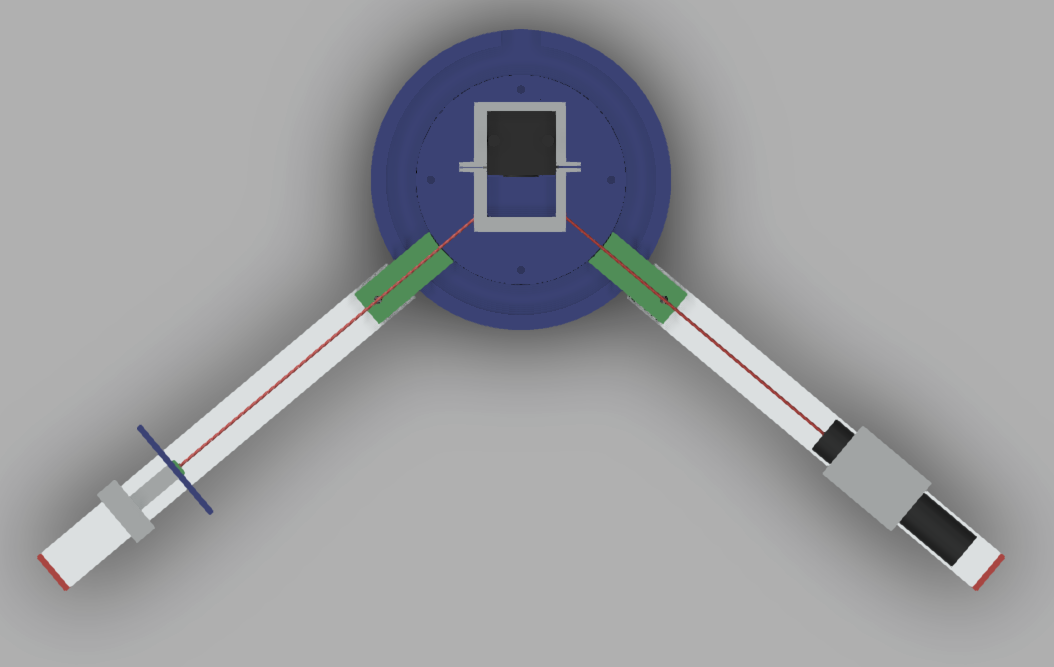
\includegraphics[width=0.7\textwidth]{experimental_setup.png}
			\caption{The laser on the right side of the image couples into the prism-multilayer structure atop the centerpiece and is then reflected into a CCD where data can be taken.}
			\label{fig:SETUP}
		\end{center}
	\end{figure}

	As fluids or gases are put into the flowcell chamber the index of refraction, $n_c$, changes. The condition for total internal reflection, found from Snell's law, for the interface between a glass prism and some transmitting medium whose index of refraction varies with time is given by:
	\[
		\sin\left({\theta_c(t)}\right) = \frac{n_c(t)}{n_g}
	\]

	We obtain an expression for the angle of reflection as a function of time by the Law of Reflection:

	\[
		\theta_r(t) = \arcsin{\frac{n_c(t)}{n_g}}
	\]

	Note that this expression is only valid for a single interface and hence does not accurately reflect our setup as we use a multilayer that behaves much differently than a single interface. With that said, this expression for $\theta_r$ does capture the essence of our setup; the reflected angle (this is equivalent to the position of the surface mode) is a dependent on the index of refraction of the chamber. Using this fact we can associate variations in the flowcell chamber's refractive index with differences in the BSWs angular position. These angular differences can be calculated by tracking the variation in the position of the dark band in the reflected image. A detailed analysis relating a shift in pixels on the CCD to the angular variation of the surface mode is listed in the methods section.

	\hspace{0.25in}
	To use this device for disease detection, or to detect any sort of biological binding process, the multilayer must have the binding agent in question deposited onto the outer layer. The characteristic of the surface mode is first captured with just the binding agent and an empty (or water filled) flowcell chamber. After acquiring the characteristic of the surface mode the molecules to be binded are then flushed through the chamber and if binding occurs the surface mode's characteristics will be different than before.
	\pagestyle{empty}
\end{flushleft}
